\chapter{Aktueller Stand der Forschung und Praxis}

\section{Ressourcenverbrauch bei KI-Modellen}
\subsection{Ressourcenverbrauch bei KI-Modellen}

substantial challenges in high consumption of computational, memory, energy, and financial resources, especially in environments with limited resource capabilities\footcite[cf.][1-2]{baiEfficiencySystematicSurvey2024}

\subsubsection{Nachhaltigkeit}
\subsubsection{Stromverbrauch}
\subsubsection{Rechenleistung begrenzt, KI-Modelle wachsen schneller als verfügbare Leistung}

\section{Neural Networks - Boltzmann Machines}

Over the past few years, the emergence of artificial neural networks has transformed
the field of computer vision and extended its influence to other areas. These include natural language processing,
game strategy development and execution (with examples in playing Atari and Go),
and optimization of navigation tasks, such as determining the most efficient routes on maps.\footcite[cf.][305]{cichyDeepNeuralNetworks2019}
Therefore, it is fair to say that neural networks are part of various important applications.\footcite[cf.][1513]{gawlikowskiSurveyUncertaintyDeep2023}
Particularly in the last two years, artificial intelligence has also garnered widespread interest from the public, especially regarding chatbots like ChatGPT and Google Bard.\footcite[cf.][1-2]{singhChatGPTGoogle2023}  
An important feature of a neural network-based system that are inspired by our brain, is that they can learn and adapt to data.\footcite[cf.][305]{cichyDeepNeuralNetworks2019}

Internally, neural networks are computational models that consist of many simple processing units, called neurons that work together in parallel often structured within interconnected layers.\footcite[cf.][305]{cichyDeepNeuralNetworks2019}
They consist out of a network architecture, which describes the layout and how the neurons are wired. Secondly, they have a optimization function which specifies the goals persued in the learning process.\footcite[cf.][1583]{durstewitzDeepNeuralNetworks2019}
Lastly, there is a training algorithm that varies all of the hyperparameters, like connection strengths between neurons, training iterations, the learning rate, etc..\footcite[cf.][1583]{durstewitzDeepNeuralNetworks2019}
The following figure 1 shows a typical neural network that consists out of a input layer, a hidden layer and an output layer with dots representig the neurons wirthin the network.
\begin{figure}[H]
    \centering
    \fbox{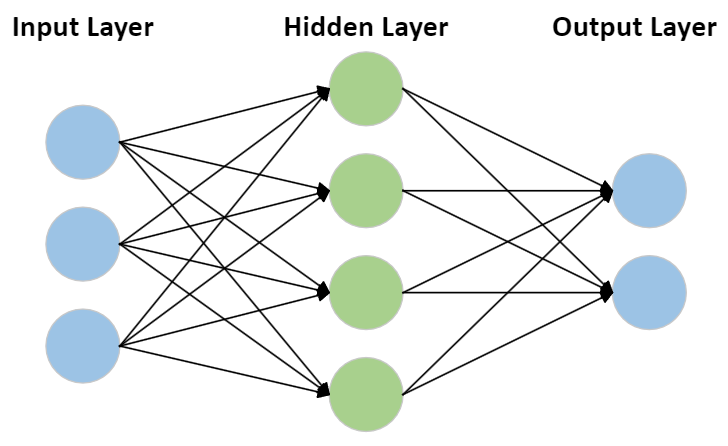
\includegraphics[width=0.55\linewidth]{graphics/Neural_Network.png}}
    \caption{figure of a neural network}
\end{figure}
Although, when these interconnected layers are stacked on top of each other, so multiple hidden layers are stacked on top of each other, the network is called deep.\footcite[cf.][305]{cichyDeepNeuralNetworks2019}
In general, deep learning methods can be seen as subset of machine learning methods and are today's fundament of artificial intelligence allowing to solve more complex tasks.\footcite[cf.][1583]{durstewitzDeepNeuralNetworks2019}
\ac{DNN}s are constantly growing and currently have around 1200 interconnected layers that equal to more than 16 million neurons inside a network .\footcite[cf.][2]{mallComprehensiveReviewDeep2023}
An example of a deep neural network is presented in figure 2 which shows the stacked layers in the middle of the network.
\begin{figure}[H]
    \centering
    \fbox{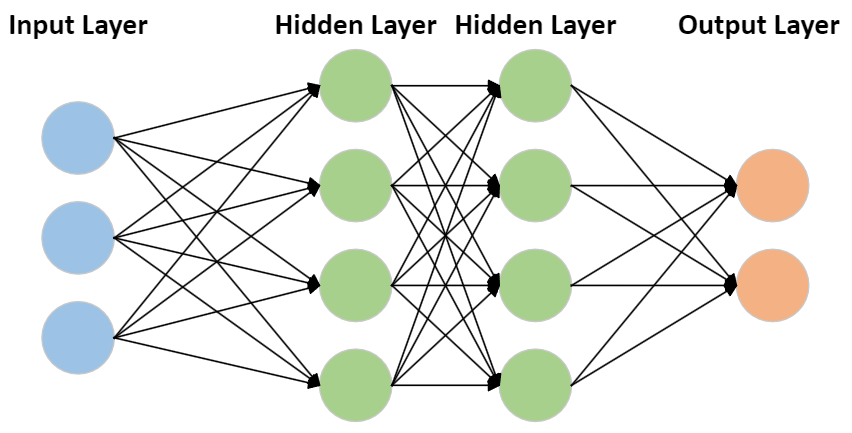
\includegraphics[width=0.6\linewidth]{graphics/Deep_Neural_Network_2.png}}
    \caption{figure of a neural network}
\end{figure}

Some examples for regression tasks within a \ac{DNN} in the field of acomputer vision include object detection, medical image registration, head- and body-pose estimation, age estimation and visual tracking.\footcite[cf.][325-326]{gustafssonEnergyBasedModelsDeep2020}
Nowadays, verly large neural networks with millions of parameters can be created due to the research achievements made in the field of neural networks and deep learning leading to highly performing models.\footcite[cf.][152]{marinoDeepNeuralNetworks2023}
Nonetheless, such models often have a negative effect on the environment in terms of unnecessary energy consumption and a limitation to their deployment on low-resource devices because they are excessively oversized and redundant.\footcite[cf.][152]{marinoDeepNeuralNetworks2023}


\subsection{Energy-based models}

An \ac{EBM} is a type of neural network that has special characteristics. 
One characteristic is that an \ac{EBM} is a statistical model.\footcite[cf.][2]{huembeliPhysicsEnergybasedModels2022}
This probabilistic approach willingly uses uncertainty into the model calculations to draw the models inputs randomly from its underlying distribution.\footcite[cf.][25-27]{uusitaloOverviewMethodsEvaluate2015}
This is done because the conventional deterministic method of backpropagation is known to potentially convert to local minimas, and requires long computation time.\footcite[cf.][109]{spechtProbabilisticNeuralNetworks1990}
As a result with conventional backpropagation more frequently incorrect classification would take place.
The second characteristic is that an \ac{EBM} is determined by an energy function that needs to be minimized in order to find the solution of the optimization problem.\footnote{cf.\cite{huembeliPhysicsEnergybasedModels2022}, p. 2; cf.\cite{ranzatoEfficientLearningSparse2006}, p. 1}
Since 1982, those statistical neural network models have been continuously emerging in the machine learning field when J.J. Hopfield introduced the Hopfield Network.\footcite[cf.][]{hopfieldNeuralNetworksPhysical1982}
Current developments include their use in reinforcement learning, potential replacements for discriminators in generative adversarial networks and for quantum \ac{EBM}s.\footnote{cf.\cite{verdonQuantumHamiltonianBasedModels2019}, p. 1; cf.\cite{duModelBasedPlanning2021}, p. 1}
In addition to that, Open AI showed that \ac{EBM}s are useful models across a wide variety of tasks like achieving state-of-the-art out-of-distribution classification and continual online class learning to name a few.\footcite[cf.][1-2]{duImplicitGenerationGeneralization2020}
The underlying idea behind \ac{EBM}s is to establish a probabilistic physical system that is able to learn and memorize patterns but most importantly generalize it.\footcite[cf.][2]{huembeliPhysicsEnergybasedModels2022} 
Especially, it involes learning an energy function \(E_{\theta}(x) \in \mathbb{R}\), with \( x \) representing the configuration of the network, and assigning the low energy to observed data \(x_i\) and high energy to other values \(x\).\footcite[cf.][330]{gustafssonEnergyBasedModelsDeep2020}
\begin{figure}[H]
    \centering
    \fbox{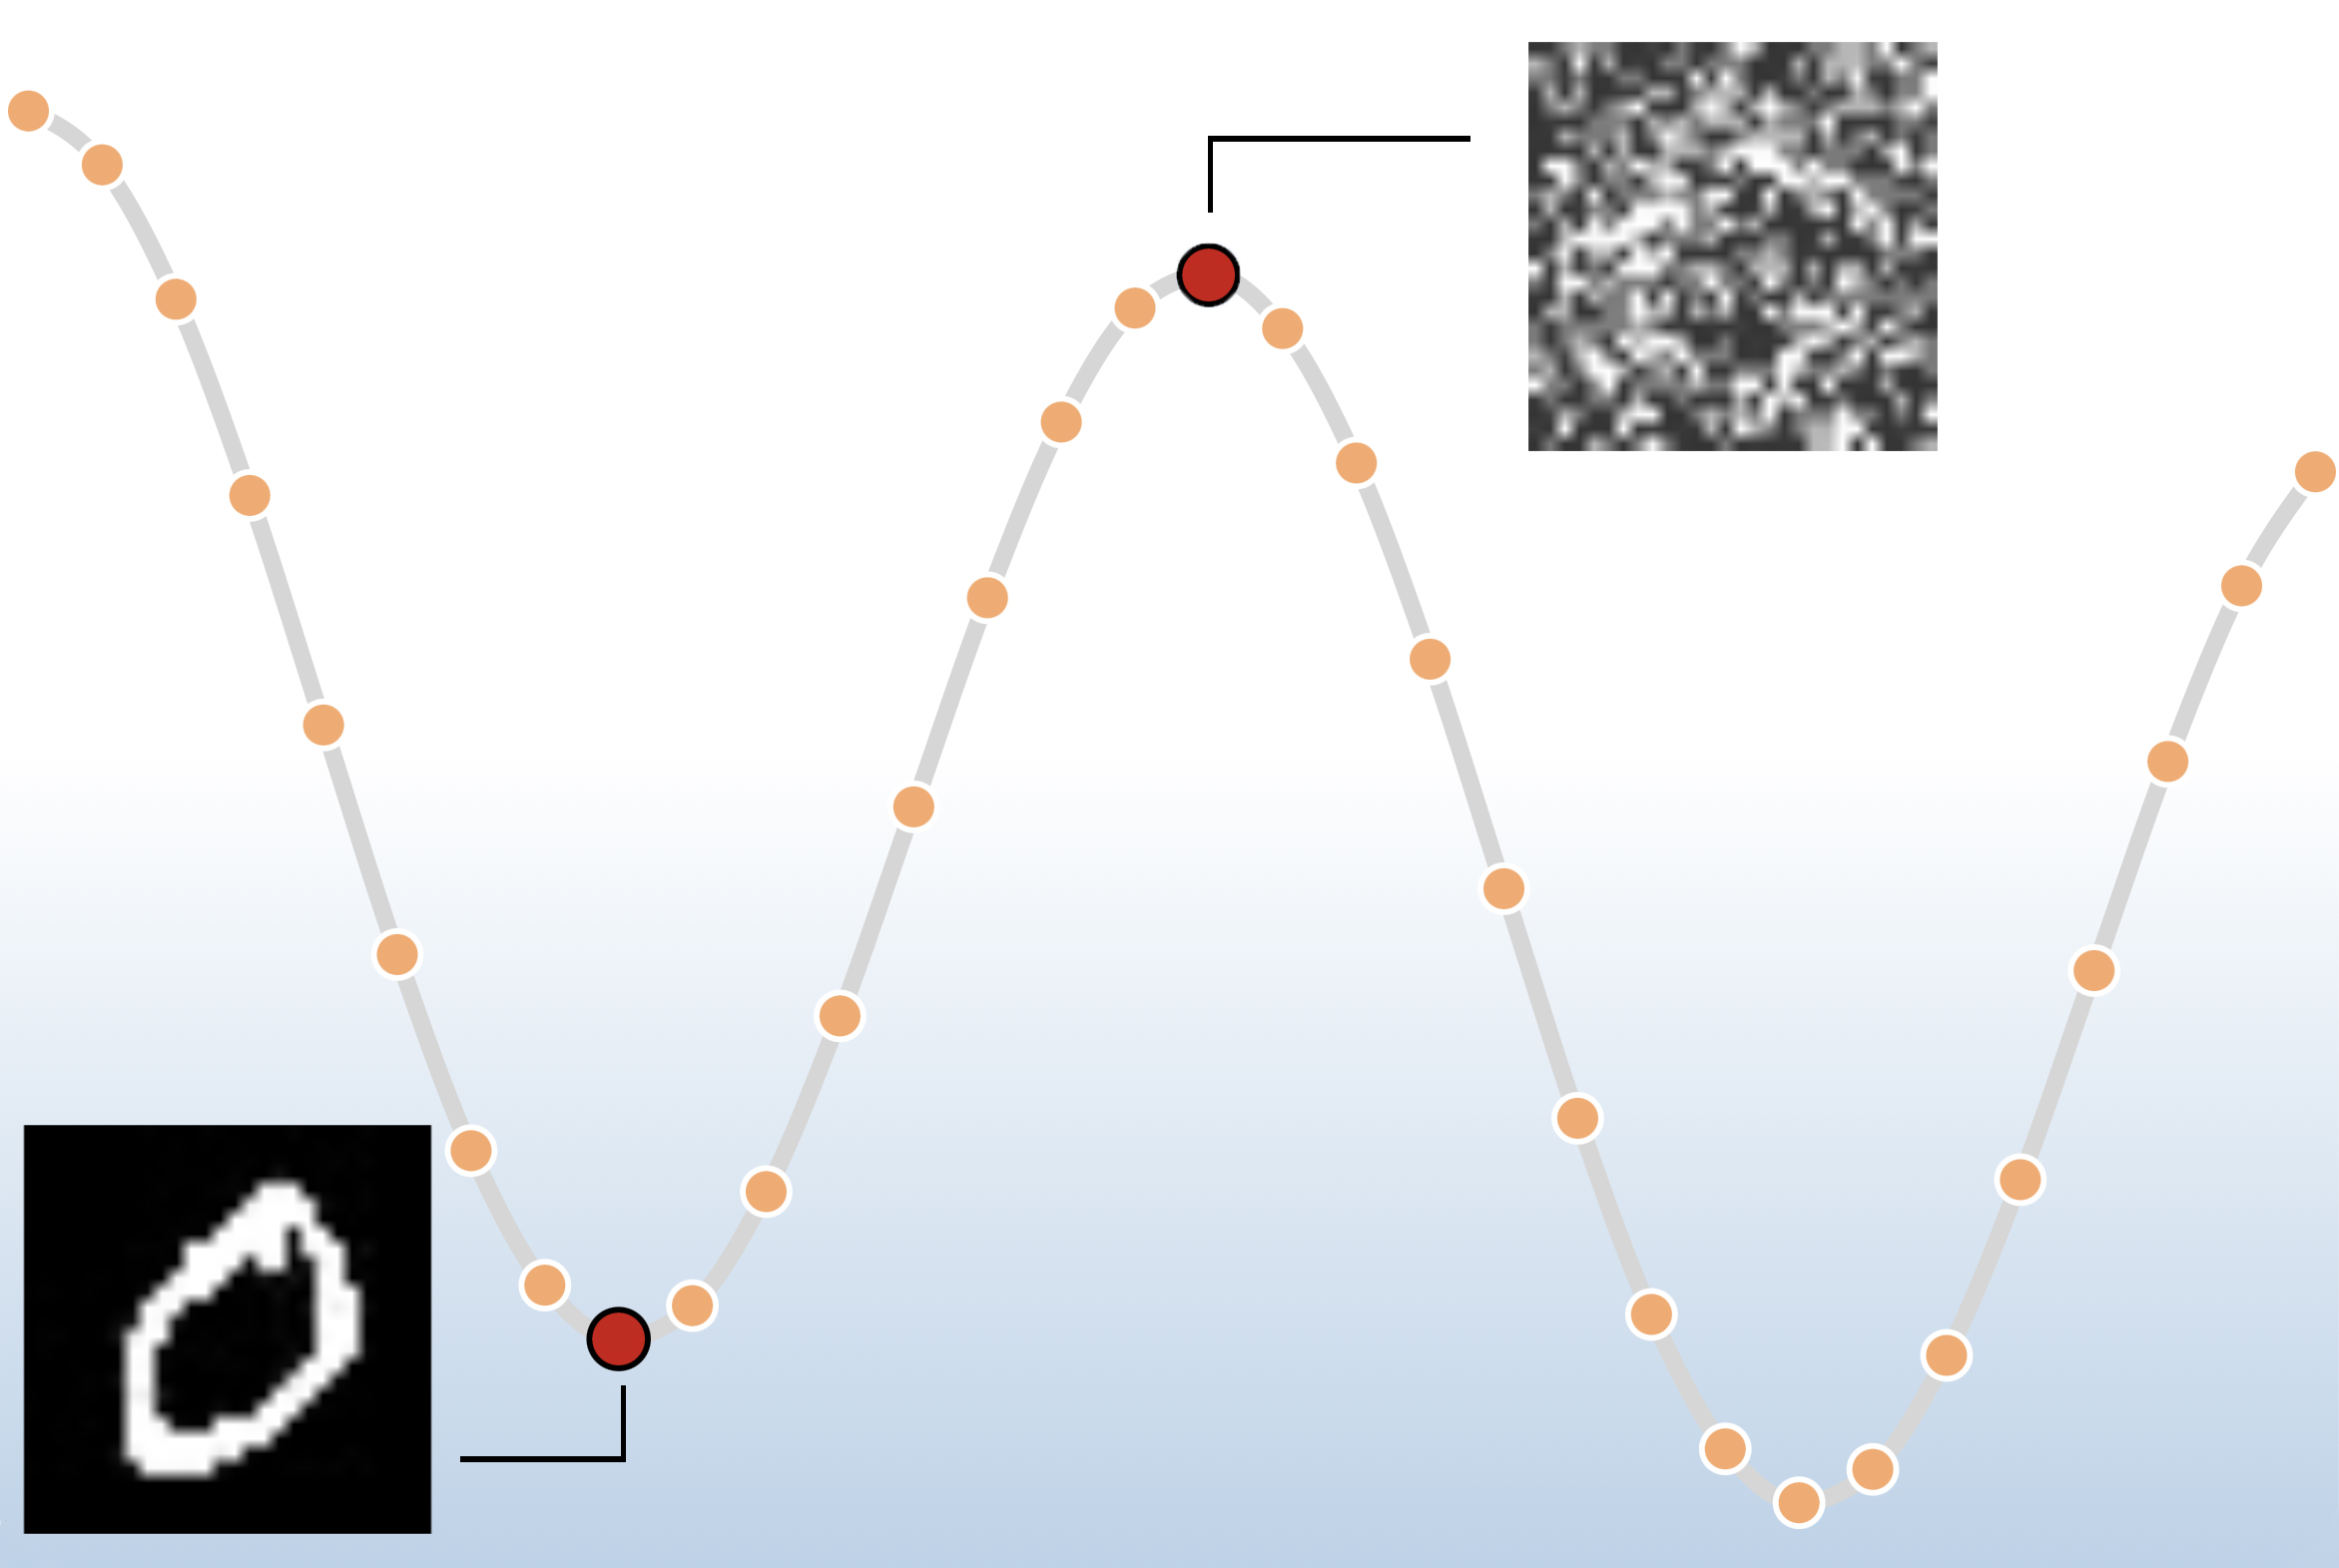
\includegraphics[width=0.4\linewidth]{graphics/energielandschaft.jpg}}
    \caption{Figure of a simplified energy landscape}
\end{figure}
In this figure 1 a simplified energy landscape is shown where the local minima corresponds to states that encode an MNIST digit.\footcite[cf.][6]{huembeliPhysicsEnergybasedModels2022} It is visible that observed data settles in the local minimum of the energy landscape, in this case a clear 0. On the other hand close to the local maxima of the energy landscape the 0 is only barely recognizable and therefore got a higher energy value assigned to it.
The assumption of the underlying distribution function \( P(x) \) represents the probability distribution over the input data x,
indicating how likely different configurations of x are under the models learned patterns:
\begin{equation}
    P(x) = \frac{1}{Z} \exp\left(-\frac{E(x)}{T}\right),
\end{equation}
where \( Z \) is the partition function to ensure
that the density function normalizes to a total probability of 1 and \( T \) is interpreted as the temperature.\footcite[cf.][2-3]{huembeliPhysicsEnergybasedModels2022}
The partition function \( Z \) used in 2.1 is given by summing over all possible pairs of visible and hidden vectors\footcite[cf.][4]{hintonPracticalGuideTraining2012}:
\begin{equation}
    Z = \sum_x \exp\left(-\frac{E(x)}{T}\right)
\end{equation}
The aim of the training in an \ac{EBM} is to match the true probability distribution \( P_{\text{data}} \) as closely as possible with the internal probability distribution \( P_{\text{model}} \) learned by the model.
What this means is that the specific aim is to adjust its parameters such that \( P_{\text{model}} \)
becomes as close to \( P_{\text{data}} \) as possible, which shows the model has learned the distribution of the real world data.
A practical method to achieve this goal is to use the KL divergence. KL divergence is a mathematical meassure that helps to meassure how close the predictions are by comparing the model's learned distribution to the true distribution of the data:
\begin{equation}
    G = \sum_x P_{\text{data}}(x) \ln \left( \frac{P_{\text{data}}(x)}{P_{\text{model}}(x)} \right)
\end{equation}
Here, \( P_{\text{data}} \) is the probability distribution when the network receives a speicific data input from the environmnet, while \( P_{\text{model}} \) represents the internal network running freely, also referred to as ``dreaming''.\footcite[cf.][154-155]{ackleyLearningAlgorithmBoltzmann1985}
In the training process the asymmetric divergence \( G \) needs to be miminized and therefore the probabiliies of the model converge close to the ones in reality.
To optimise the KL divergence the energy is adjusted, whereby data is assigned to low energy states (according to 2.1) and the training data receives high energy and therefore low probabiliies.\footcite[cf.][2-3]{zhaiDeepStructuredEnergy2016}

NACH UNTEN
As a side note it is worth mentioning that using the maximum likelihood estimator for \( Z \) is intractable due to the requirement of summing over all possible states, which leads to an exponential increase in the number of states for larger systems.\footcite[cf.][2-3]{zhaiDeepStructuredEnergy2016}

\subsection{concept of Boltzmann Maschines}

A \ac{BM} is a type of symmetrical \ac{EBM} consisting of binary neurons \{0, 1\}.\footcite[cf.][260]{amariInformationGeometryBoltzmann1992}
The neurons of the network can be split into two functional groups, a set of visible neurons and a set of hidden neurons.\footcite[cf.][154]{ackleyLearningAlgorithmBoltzmann1985}
Therefore, the \ac{BM} is a two-layer model with a visible layer (``v'') and a hidden layer (``h'').\footcite[cf.][448]{salakhutdinovDeepBoltzmannMachines2009}
The visible layer is the interface between the network and the environment. It receives data inputs during training and sets the state of a neuron to either \{0, 1\} which represents activated or not activated.
On the other hand, the hidden units are not connected to the environment and can be used to explain underlying constraints in the internal model of input vectors and they cannot be represented by pairwise constraints.\footcite[cf.][154]{ackleyLearningAlgorithmBoltzmann1985}
The connection between the individual neurons is referred to as bidirectional, as each neuron communicates with each other in both directions.\footcite[cf.][149]{ackleyLearningAlgorithmBoltzmann1985}
As early as 1985, one of the founding fathers of artificial intelligence, Geoffrey Hinton, was aware that an \ac{BM} is able to learn its underlying features by looking at data from a domain and developing a generative internal model.\footcite[cf.][148]{ackleyLearningAlgorithmBoltzmann1985}

Most machine learning models can be categorized in either generative or discriminative models. Both are strategies to estimate a probability that an specific object can be assigned to a category.\footcite[cf.][1]{hsuEffectsGenerativeDiscriminative2010}
Discrimivative models estimate the probability distribution based on category labels that are given to specific objects.\footcite[cf.][2]{gmComprehensiveSurveyAnalysis2020}
On the other hand, a generative model differ as follows. 
They generate a probabilistic model of the underyling probability distribution for each category, which is assumed as the basis of the data, and in a following step they use Baye's rule to identify which category is very likely to have establihed the object.\footcite[cf.][1]{hsuEffectsGenerativeDiscriminative2010}
An real world example would be the following: to predict if a movie will be a hit, you could analyze past box office successes to model characteristics shared by hits (generative approach), or assess immediate audience reactions to movie trailers and reviews to predict success without modeling historical data (discriminative approach).
Therefore it can be said that \ac{BM}s and \ac{EBM}s are generative models. In the following figure \ref{fig1}, a general \ac{BM} is depicted, where the upper layer embodies a vector of stochastic binary 'hidden' features, while the lower layer embodies a vector of stochastic binary 'visible' variables.\footcite[cf.][449]{salakhutdinovDeepBoltzmannMachines2009}

\begin{figure}[H]
    \centering
    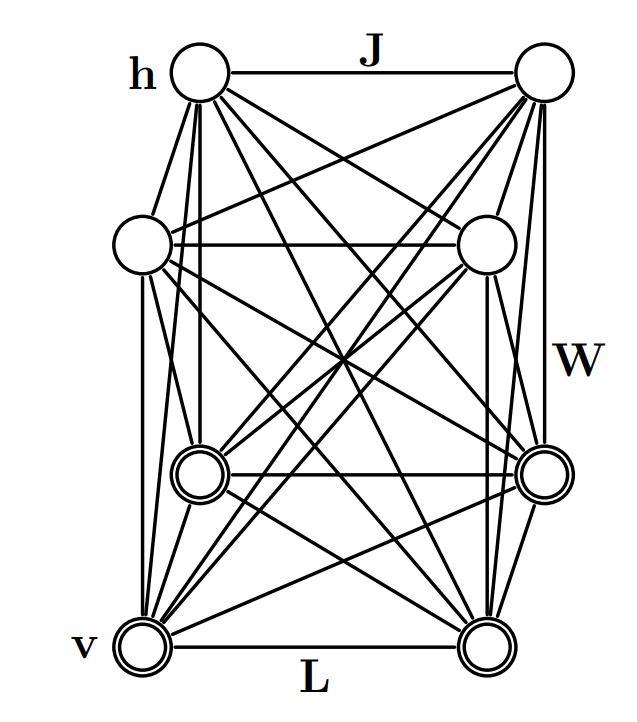
\includegraphics[width=0.25\linewidth]{graphics/General_BM.png}
    \caption{figure of a general Boltzmann Machine}
    \label{fig1}
\end{figure}
The model contains a set of visible units \( v \in \{0, 1\} \), and a set of hidden units \( h \in \{0, 1\} \) (see Fig. 1). The energy function of the \ac{BM} with the states \( \{v, h\} \) is defined as:
\begin{equation}
E(v, h; \theta) = -\frac{1}{2} v^T L v - \frac{1}{2} h^T J h - v^T W h,
\end{equation}

where \( \theta = \{W, L, J\} \) are the model parameters.\footcite[cf.][448]{salakhutdinovDeepBoltzmannMachines2009}
\( W, L, J \) represent visible-to-hidden, visible-to-visible and hidden-to-hidden weights.
In \ac{BM} each neurons works towards minimizing the global energy by 
entering a particular neuron configuration representing a input to the machine and the system will find the minimum energy configuration that is compatible with the given input.\footcite[cf.][150]{ackleyLearningAlgorithmBoltzmann1985}
A simple method to find a local energy minimum involes to switch into wichever of the two states (on or off) of a neuron result in a lower energy given the current state of the other neurons.\footcite[cf.][110]{fahlmanMassivelyParallelArchitectures1983}    
Integrating the function 2.4 into the earlier introduced KL-divergence 2.2 and doing gradient descend a learning rule to update the weights and biases appers.\footcite[cf.][5]{hintonPracticalGuideTraining2012}
The gradient descent algorithm is commonly used in machine learning and is an iterative technique that adjusts the model parameters (weights and biases).\footcite[cf.][11]{wangResearchApplicationGradient2021}
It progressively acquires the gradient of the energy function, methodically advancing towards the optimal solution and ultimately achieves the minimum loss function along with adjusted parameters.\footcite[cf.][11]{wangResearchApplicationGradient2021}
Consequently, this leads to the specific learning rule\footcite[cf.][5]{hintonPracticalGuideTraining2012}:
\begin{equation}
    \Delta w_{ij} = \epsilon ( \langle v_i h_j \rangle_{\text{data}} - \langle v_i h_j \rangle_{\text{model}} )
\end{equation}

The network can now update the weights ``W'' that exist between the neurons through the training rule based on the observations that served as input. \footcite[cf.][1-2]{barraEquivalenceHopfieldNetworks2012}
In this case, the square brackets represent expected values, as the training is based on the activation probability.
In addition to that, the step sizes of updates to the weights are influenced by the learning rate \(\epsilon\) within the iterative training process.

Performing exact training in this model is intractable because exact computation of the data predictions and the model predictions takes a time that is exponential in the number of hidden units.\footcite[cf.][449]{salakhutdinovDeepBoltzmannMachines2009}
When the number of hidden units is large compared to the number of visible units it is impossible to achieve a perfect model because of the totally connected network and the resulting \( 2^n \) possbilities.\footcite[cf.][154]{ackleyLearningAlgorithmBoltzmann1985}
Hereby, \( n\) represents the number of neurons in the network with each neuron being in one of the two states, the total sum of possibilities are \( 2^n \).
This leads back to the briefly mentioned constraint of equation 2.3, that is needed to calculate an activation probability of a neuron, which is required to update a weight in the training process shown in 2.5.

A specific example to demonstrate why it is intractable to calculate an activiation of a \ac{BM} is the following. A fictional \ac{BM} has 80 visible nodes and 120 hidden nodes and therefore the possbilities of states of neurons are \( 2^{200} \), which is \( 1.61 \times 10^{60}\). 
To put this into perspective, the total atoms that exist on earth are only estimated to be around \( 1.33 \times 10^{50}\).\footnote{cf.\cite{helmenstineHowManyAtoms2022}, p. 478-480; cf.\cite{schlammingerCoolWayMeasure2014}, p. 1}
That means even if it would be possible to store one information per atom it would just not be enough. 

As a result, instead of directly trying to train the model sampling methods are used that are able to estimate these activation probabiliies.
This enables the training of \ac{BM}s and \ac{RBM}s.
\subsection{Restriced Boltzmann Machines}

As a simplification of the training problem Hinton and Sejnowski proposed Gibbs sampling as an algorithm to aporoximate both expectations.\footcite[cf.][158-165]{ackleyLearningAlgorithmBoltzmann1985}
Furthermore, the intralayer connections of the model got removed and the result is the so called \ac{RBM}.
To transform an \ac{BM} into a \ac{RBM} the diagonal elements \( L \) and \( J \)  introduced earlier, are set to 0 and as a result the well-known model of a \ac{RBM} establishes shown in fig.5.\footcite[cf.][449]{salakhutdinovDeepBoltzmannMachines2009}

\begin{figure}[H]
    \centering
    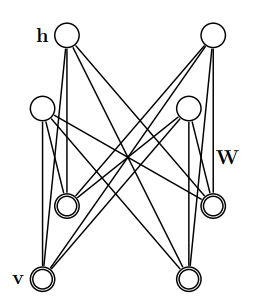
\includegraphics[width=0.25\linewidth]{graphics/RBM_Modell.png}
    \caption{Figure of a \ac{RBM}}
\end{figure}
What can be recognized that no more visible-to-visible and hidden-to-hidden connections can be found in the model.
The configuration of the visible and hidden units \( (v, h) \) therefore has also an updated energy function (Hopfield, 1982) given by:
\begin{equation}
E(v, h) = - \sum_{i \in \text{visible}} a_i v_i - \sum_{j \in \text{hidden}} b_j h_j - \sum_{i,j} v_i h_j w_{ij},
\end{equation}
where \( v_i, h_j \) are the binary states of a visible unit \( i \) and hidden unit \( j \), \( a_i \) and  \(  b_j \) are their biases and \( w_{ij} \) is the weight between them.\footcite[cf.][3-4]{hintonPracticalGuideTraining2012a}
Despite, compared to the fully connected \ac{BM}, the \ac{RBM} is less complex but the advantages of training surpasses the loss in expressivity possibilities.\footcite[cf.][4]{huembeliPhysicsEnergybasedModels2022}
The \ac{RBM} has recently been drawing attention in the machine learning community beceause of its adaption and extention for various tasks such as representational learning, document modeling, image recognition and for
serving as foundational components for deep networks including Deep Boltzmann Machines, Deep Belief Networks and hybrid models with CNNs.\footcite[cf.][1186]{zhangOverviewRestrictedBoltzmann2018}

\subsubsection{Training of \ac{RBM}s}

The training of \ac{RBM}s can be established with the use of sampling methods that estimate the activation probabilities, which are needed to update the weights.
There are currently two methods that can be chosen from: contrastive divergence and the Metropolis-Hastings algorithm. 
The goal of the techniques is to create a sequence of correlated steps from a random walk that, after enough iterations, makes it possible to sample a desired target probability distribution.\footcite[cf.][1]{patronOptimalRelaxationRate2024}
In the following part both methods will be explained in depth.
Especially, they are interesting since they serve as baselines to compare against the new sampling method of a hopfield network that is to be achieved in the practical part of the thesis.

\textbf{Contrastive Divergence:} Contrastive divergence is a special Gibbs Sampling training method
developed by Geoffrey Hinton for the efficient training of \ac{RBM}s.\footcite[cf.][4-5]{hintonPracticalGuideTraining2012}
In traditional, Gibbs sampling would have to generate a long chain of samples, until
independent samples are obtained from the observed data distribution of the model.\footcite[cf.][5-6]{huembeliPhysicsEnergybasedModels2022}
The samples are needed for each iteration of the gradient ascent on the log-likelihood
resulting in large computational costs.\footcite[cf.][7-8]{upadhyaOverviewRestrictedBoltzmann2019}
To solve this issue contrastive divergence minimizes an approximation of the Kullback-Leibler divergence between the empirical distribution of the training data and the distribution generated by the model.\footcite[cf.][246]{mocanuTopologicalInsightRestricted2016}
They way to achieve this is by initializing the Markov chain with the samples from the data distributon.\footcite[cf.][7-8]{upadhyaOverviewRestrictedBoltzmann2019}
The outcome has been shown to heavily decrease the training time while only adding a small bias.\footcite[cf.][537]{larochelleClassificationUsingDiscriminative2008}
This allows to calculate the probabilities of equation 2.5. 
This entails initializing the visible units using an actual data input, such as an MNIST sample, and then commencing the subsequent steps with the hidden states.
Often the process can be stopped after only sampling a very small number of steps.\footcite[cf.][646]{larochelleLearningAlgorithmsClassification2012}


\textbf{1. Forward Pass (positive phase)}

During the forward pass using the Gibbs Sampling method, the visible units are set to a completely random state. Next up the hidden units are computed.
The computation of the hidden units involves calculating their activation probabilities and performing an actual sampling with their calculated activation probabilities.
With the \ac{RBM} it is now easy to get an analytical calculated sample of $(\textbf{v}_i\textbf{h}_j)_{data}$.\footcite[cf.][5]{hintonPracticalGuideTraining2012}
Given an input data out of the training images, \( v \), the binary state, \( j \), of each hidden unit,  \( h_j \), is set to 1 with following probability:

\begin{equation}
p(h_j = 1 | \textbf{v}) = \sigma(b_j + \sum_i v_i w_{ij}),
\end{equation}
where $\sigma(x)$ is the logistic sigmoid function with an unbiased sample. The sigmoid function is defined as $\sigma(x) = \frac{1}{1 + \exp(-x)}$ and is needed because it is the underlying activation function of each neuron.
A visual representation is shown in figure 6:
\begin{figure}[H]
    \centering
    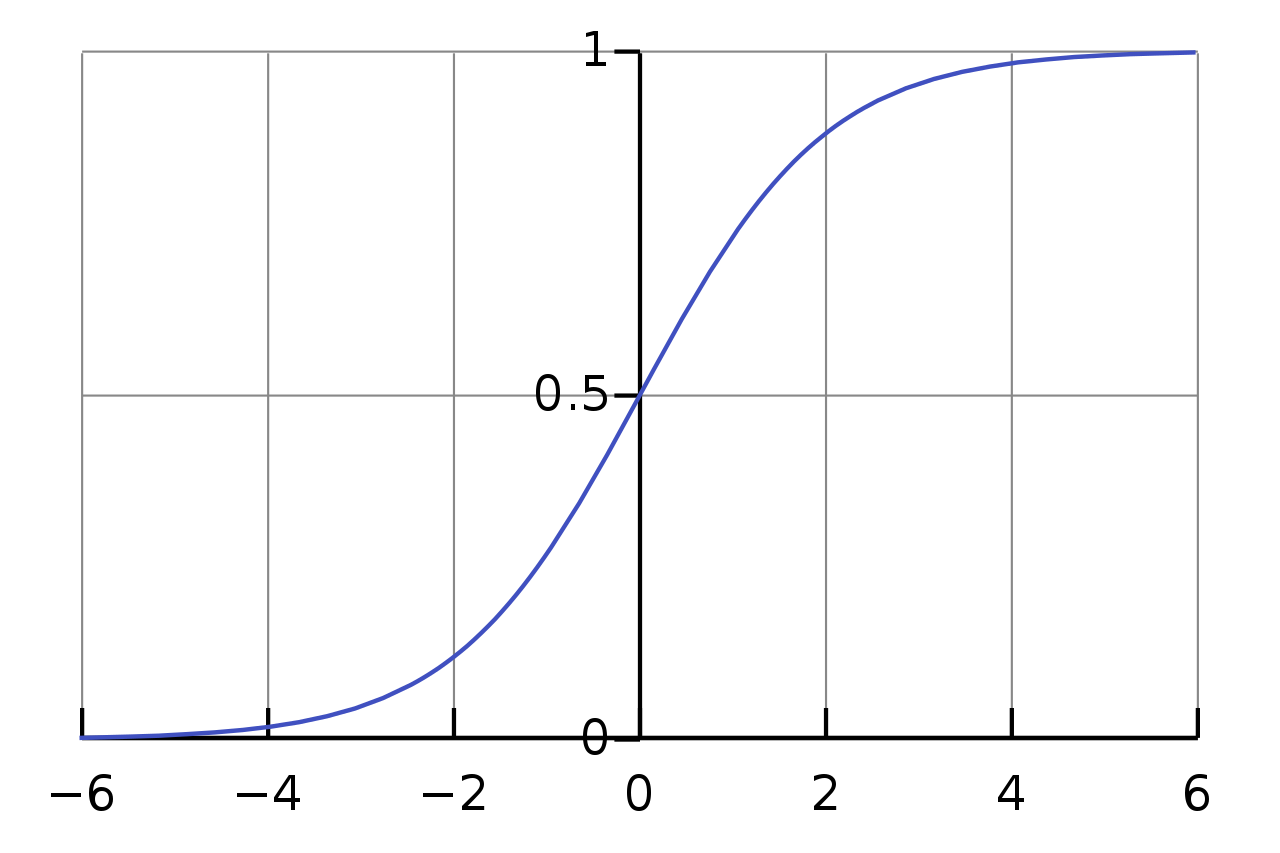
\includegraphics[width=0.5\linewidth]{graphics/logistic_sigmoid.png}
    \caption{Figure of a logistic sigmoid function \ac{RBM}}
    \label{logistic_sigmoid}
\end{figure}
The result is a set of probabilities that reflect how likely it is for each hidden unit to be on, wich stands for \( 1 \), or, which stands for \( 0 \), given the input data.\footcite[cf.][6]{huembeliPhysicsEnergybasedModels2022}
The sampling part of the positive phase uses the just calculated activation probabiliy of each hidden unit and performs a random experiment with it.
That random experiment generates a uniform random number between 1 and 0 and if the random number is greater than the just calculated activiation probability the hidden unit is set to activated.
Afterwards, the hidden unit is either activated or not activated and the training process continues with the new state of the hidden units.

\textbf{2. Reconstruction (negative phase)}

In this phase, the sampled hidden states are used to reconstruct the visible units. 
This is essentially a prediction of the input, which is how the model sees the input based on the just updated hidden units and is calulated with following probability:\footcite[cf.][6]{hintonPracticalGuideTraining2012}
\begin{equation}
    p(v_i = 1 | \mathbf{h}) = \sigma(a_i + \sum_j h_j w_{ij})
\end{equation}
The sampling part of the negative phase uses the just calculated activation probabiliy
of each visible unit and performs a random experiment, like in the positive phase.
Now, the result is a prediction of the input in the visible nodes.
Afterwards, a half forward pass is made to calculate the activation probability of a hidden unit again based on the activated or not activated visible units.

\textbf{3. Updating the weights}

Now, all the requirements to update the weights are satisfied and can be used within the equation 2.5. 
The delta that results is summed to the current weight and the internal model gets closer to prediciting the observed data.
In total, one training iteration consists out of 1 Forward Pass, 1 Reconstruction and 0.5 Forward Pass again is accomplished.
Repeating this training steps \( N \) times for a suitable chosen \( N \) the model learns better, since more steps of alternating Gibbs sampling were performed.\footcite[cf.][6]{huembeliPhysicsEnergybasedModels2022}


\textbf{Metropolis-Hastings:} The Metropolis-Hastings algorithm, often only called Metropolis algorithm, is a technique out of \ac{MCMC} class techniques.\footcite[cf.][1]{patronOptimalRelaxationRate2024}
The Metropolis-Hastings method was invented by Metropolis et al. in 1953 when they noticed, that for an intractable distribution with too many states it can be seen as a limiting distribution of Markov chains.\footcite[cf.][1087-1092]{metropolisEquationStateCalculations1953} 
The intractable distribution to handle with the Metropolis-Hastings technique in the case of \ac{RBM}s is equation 2.3.
An Interpretation of the method can be expressed as: "A visitor to a museum that is forced by a general blackout to watch
a painting with a small torch.
Due to the narrow beam of the torch, the person cannot get a global view of the painting but can proceed along this painting until all parts have been seen."\footcite[cf.][2]{robertMetropolisHastingsAlgorithm2016}
The version already adjusted for \ac{RBM}s incorporates the following functionality of the Metropolis technique:

First, select a random or given configuarion $x_{\text{old}}$ of a \ac{RBM} that holds the states of all visible and hidden neurons.\footcite[cf.][65]{beichlMetropolisAlgorithm2000}
Secondly, the energy of the configuration, noted as  $E_{\text{old}}$, must be calculated using Equation 2.6, as previously introduced. Subsequently, this energy value is stored.
Thirdly, the configuration gets updated by picking one random neuron and changing the state of it from 0 to 1 or vice versa.\footcite[cf.][1]{rosenthalOptimalProposalDistributions2009}
This new configuration is stored as $x_{\text{new}}$. Following that the energy of the new configuration $E_{\text{new}}$ is calculated and stored.
Now the two energy values are compared and if $E_{\text{new}}$ <= $E_{\text{old}}$ the new configuration will be accepted and $x_{\text{old}}$ = $x_{\text{new}}$.\footcite[cf.][1-2]{patronOptimalRelaxationRate2024}
If $E_{\text{new}}$ > $E_{\text{old}}$ then there are some extra steps to be followed: 

The flip probability is calculated as $p=\exp\left(-\frac{E_{\text{new}}-E_{\text{old}}}{kT}\right)$.
\( KT \) is interpreted as the temperature in the network and with higher temperature it increases
the activation probability leading to an faster exploration through the landscape but with less details.\footcite[cf.][1-9]{liTemperatureBasedRestricted2016}
For \ac{RBM}s \( KT \) is assumed to be 1.\footcite[cf.][3]{hintonBoltzmannMachines2014} In the following figure 7 the resulting probability function is shown.

\begin{figure}[H]
    \centering
    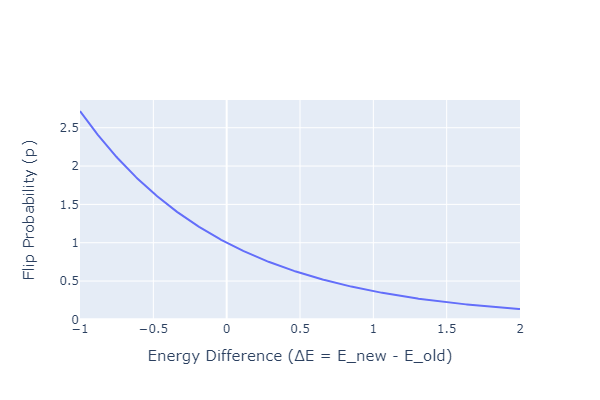
\includegraphics[width=0.7\linewidth]{graphics/Flip Probability Function in Metropolis-Hastings Algorithm2.png}
    \caption{Flip Probability Function in Metropolis-Hastings Algorithm}
\end{figure}

In the next step a uniform random number $r$ between 0 and 1 is generated.
After generating $r$ the configuration will be accepted if $r \leq p$ (i.e., $x_{\text{old}}=x_{\text{new}}$).\footcite[cf.][2-3]{patronOptimalRelaxationRate2024}
Otherwise, a rejection takes place if $r > P$ (i.e., $x_{\text{old}}=x_{\text{old}}$).

Finally, the configuration $x_{\text{old}}$ can be stored and the process repeats beginning from step 2 on.\footcite[cf.][17]{patronOptimalRelaxationRate2024}
After repeating enough times the activation probability for each neuron can be calculated by summing over all samples $(x_1+x_2+x_3+\ldots)$ and the result is divided by the total number of samples.

\subsection{Current Problems witht BMs and RBMs}

One general problem that occurs in the learning process of a \ac{BM} is that it is both time-consuming and difficult.\footcite[cf.][1-2]{fischerIntroductionRestrictedBoltzmann2012}
This is because sampling from an undirected graphical model is not straightforward and therefore \ac{RBM}s make use
of \ac{MCMC} proposed methods like Contrastive Divergence and Metropolis Hastings.\footcite[cf.][2]{fischerIntroductionRestrictedBoltzmann2012}
In addition to that, the selection of hyperparameters can be difficult since for the training of a practical model a large hyper-parameter space needs to be explored.\footcite[cf.][536]{larochelleClassificationUsingDiscriminative2008}
Hyperparmeters are: the learning rate, size of the hidden layer, number of training iterations iteration count per bias (sampling step size), initializing the weight sizes in the beginning but also the method for calculating activation probabilities (Contrastive Divergence, Metropolis Hastings, etc.).
As a result, establishing a \ac{RBM} with perfect hyperparameters is time consuming and can be seen as art.
Furthermore, training can become unstable and predictions become inaccurate due to an incompatible selected temperature.\footcite[cf.][3-4]{huembeliPhysicsEnergybasedModels2022}
A lower temperature reduces the system's possbility to explore the energy landscape thoroughly, leading to the false selection of local minima instead of finding the global minimum.
Vice versa a too high temperature can cause that the energy landscape is not explored enough and has gaps between it missing some minima or skipping the global maxima. 
Luckily, the temperature for \ac{RBM}s is expected to be \( 1 \) and only for specific use cases it makes sense to adjust internal temperature.

To accelerate the training process of a \ac{RBM}, it is crucial to address the most computationally demanding aspect: the matrix-vector multiplication involved in the sampling process.
A possbilty of achieving this is using dedicated hardware, so called hardware accelerators for this problem. 
They are designed to tackle a specific task very efficiently, like matrix vector multiplications, which are widely used within most of the neural networks.\footcite[cf.][3881-3882]{lehnertMostResourceEfficient2023}
That is the reason why they are significant for the acceleration of this thesis and an interesting technology to look at.  


\section{Hardware accelerators}
\subsection{Current approaches in the field of AI and other solutions}
Since Neural Networks and \ac{DNN}s are growing their parameters at rapid rates they constantly achieve better and better resutls and are able to solv even more complex tasks.\footcite[cf.][1]{baischerLearningHardwareTutorial2021}
This upcoming trend of growing network sizes exponentially also brings a dark side with it: An excessive increase in computational effort and memory size.\footcite[cf.][1-2]{baischerLearningHardwareTutorial2021}
As a result \ac{CPU}s can barely satisfy the required performance and specialized hardware accelerators are used to increase the performance of these Neural Networks.\footnote{cf.\cite{zhouPhotonicMatrixMultiplication2022}, p. 1-2; cf.\cite{baischerLearningHardwareTutorial2021}, p. 2}
In addition to that for many use cases, like autonomous driving, there are high energy, latency, and runtime predictability constraints \ac{CPU}s are not able to meet.\footcite[cf.][2692]{ahmadOptimizingHardwareAccelerated2020}

The concept of developing hardware accelerators is not new.
However, their limited adoption and the fast obsolescence of even the most outstanding accelerators have made the investment in them uneconomical compared to general-purpose processors that surpassed them.\footcite[cf.][2]{peccerilloSurveyHardwareAccelerators2022}
At present, however they are seen as promising driving force of computer architecture since they are the optimal solution to satisfy the growing computation-hungry demands of businesses, especially within machine learning workloads.\footcite[cf.][2-3]{peccerilloSurveyHardwareAccelerators2022}
An hardware accelerator can be defined as "a separate architectural substructure that is architected using a different set of objectives than the base processor, where these objectives are derived from the needs of a special class of applications".\footcite[cf.][2]{peccerilloSurveyHardwareAccelerators2022}
Broken down, they are specialized hardware, expertly optimized for the unique demands of certain application categories, freeing them from the restrictions usually placed on general-purpose processors.
Moreover, a hardware accelerator doesn't replace the conventional processor, which is still used for the operating system, it rather enables specific workloads to be executed on it very efficiently.\footcite[cf.][2-3]{peccerilloSurveyHardwareAccelerators2022}
There are different approches such as \ac{GPU}s, \ac{ASIC}s, \ac{FPGA}s, but also new approaches like Quantum Computations or Photonic matrix multiplication are researched.\footnote{\cite{zhouPhotonicMatrixMultiplication2022}, p. 1-2; cf.\cite{baischerLearningHardwareTutorial2021}, p. 2}
All of these methods have different use cases and get more and more application specific. The list of the sequence, sorted by application-unspecific to specific for established approches looks the following:
\[
\text{CPU} \xrightarrow{\text{less flexible}} \text{GPU} \xrightarrow{\text{specialized}} \text{FPGA} \xrightarrow{\text{more customized}} \text{ASIC}
\]
Currently the approaches can be segmented into three categories:
\textbf{Firstly}, the design of data-driven digital circuits.
It consists the shift from general-purpose GPUs to specialized dataflow architectures like systolic arrays, which are used in Google’s Tensor Processing Units (TPUs).
These architectures are noted for their efficiency in performing deep learning operations by reducing control hardware and keeping data movement local.\footcite[cf.][3883]{lehnertMostResourceEfficient2023}
\textbf{Secondly}, network structure optimizations. 
Hereby modifications to the neural networks themselves are made to improve hardware efficiency.
One method is quantization, which simplifies arithmetic operations and reduces memory needs by using fixed-point representations of data and weights instad of using for example 32-bit floating points.
The other one is pruning, which involves setting certain weights to zero to reduce the complexity of operations.\footcite[cf.][3883]{lehnertMostResourceEfficient2023}
\textbf{Thirdly}, technology-driven designs.
Current research into using novel circuitry and memory cells include memristive memory cells and silicon photonics, to further enhance performance and energy efficiency.
They work by storing the network weights and calculating the vector multiplications with analaog signals with technologies like crossbar arrays.
While these technologies promise significant advantages, their practical application is still being explored.\footcite[cf.][3883]{lehnertMostResourceEfficient2023}
The following three accelerator approaches can be categorized into the first category:

\subsection{GPU}
The \ac{GPU}, is by far the most common accelerator in the market with a focus at computational-complex workloads.
Also \ac{GPU}s enabled great achievements in \ac{DNN}s due to their massive parallelization potential of computations and their high troughputs compared to \ac{FPGA}s and \ac{ASIC}s.\footcite[cf.][16]{baischerLearningHardwareTutorial2021}
A \ac{GPU} is a manycore unit that features up to hundreds of multi-processors that consist of in-order cores which are able to exploit massive threadlevel parallelism.\footcite[cf.][2]{peccerilloSurveyHardwareAccelerators2022}
They excel at performing numerous floating-point arithmetic operations for vector processing on large datasets with high degrees of data-parallelism.
In practice this works by breaking down workloads into small tasks that can be processed by the enormous amount of cores in parallel.\footcite[cf.][101]{huSurveyConvolutionalNeural2022} 
With development of real-time graphics \ac{GPU}s became programmable too. The combination of programmability and floating-point performance
make them very attractice for machine learning workloads and is the reson for their dominance in the market.\footcite[cf.][42]{dallyEvolutionGraphicsProcessing2021}
On top of that, the widespread adoption of \ac{GPU}s has led to extensive support across numerous frameworks and high-level APIs commonly used in Machine Learning.\footcite[cf.][16]{baischerLearningHardwareTutorial2021}
Well-known frameworks would be PyTorch or TensorFlow.
However, compared to the other two accelerator apporaches the \ac{GPU} is not as flexible and has higher latency and energy consumption.\footcite[cf.][100]{huSurveyConvolutionalNeural2022}

\subsection{Field programmable gate arrays}
In contrast, \ac{FPGA}s have also demonstrated enormous parallelization capabilities due to their fast digital signal processors and on-chip
memory which result in lower energy cost than GPUs.\footcite[cf.][2693]{ahmadOptimizingHardwareAccelerated2020}
They work by using reconfigurable logic blocks that can be interconnected using routing tracks with configurable switches at the intersections.\footcite[cf.][144]{babuReconfigurableFPGAArchitectures2021}
This combined with the use of many digital signal processors and local storage of data in the hardware enables the development of the exact hardware needed for a workload.\footcite[cf.][19]{baischerLearningHardwareTutorial2021}
As a side note it is worth mentioning that the most energy-consuming task of a workload is the data transfer and not the computation iself.
In the context of \ac{FPGA}s, they use their on-chip memory to reduce the data transfer significantly and therefore achieve a sweet spot between computation speed and energy efficiency.\footcite[cf.][101-102]{huSurveyConvolutionalNeural2022}
Hence, they are utilized to design a specialized processor tailored for executing specific workloads, like machine learning, effectively.\footcite[cf.][322]{sipolaArtificialIntelligenceIoT2022}
Furthermore, due to their reprogrammable nature they have a lower engineering cost and faster time-to-market compared to \ac{ASIC}s.\footcite[cf.][4]{boutrosFPGAArchitecturePrinciples2021}
With \ac{FPGA}s the implementation time could only be a matter of weeks and also allows to support continious upgrades and bug fixes even after the deployment which is not possible within \ac{ASIC}s\footcite[cf.][4]{boutrosFPGAArchitecturePrinciples2021}
Even though the \ac{FPGA} possesses all these advantages with their high flexibility, latency and low energy consumption, they are sometimes inferior in throughput compared to a \ac{GPU}.\footcite[cf.][100]{huSurveyConvolutionalNeural2022}

\subsection{Application specific integrated circuit}
\ac{ASIC}s can be distinguished from \ac{FPGA}s because they are not programmable. 
In addition to that, they offer the highest degree of customization and are designed to execute a specific application with the utmost efficiency.\footcite[cf.][17]{baischerLearningHardwareTutorial2021}
So the attributes of \ac{ASIC}s are the focus on specific tasks and the strong design freedom.
Nowadays, the most common type of \ac{ASIC}s are \ac{TPU}s because of their matrix vector multiplications abilities that are needed within machine learning. But conventional \ac{ASIC}s work by mapping neurons directly to the hardware.\footcite[cf.][104]{huSurveyConvolutionalNeural2022}
Their design architecture enables them to outperform \ac{GPU}s and \ac{FPGA}s in terms of their small size, greater computation speed and high power efficiency.\footcite[cf.][17]{baischerLearningHardwareTutorial2021}
Specifically when compared to corresponding \ac{FPGA} circuits  \ac{ASIC}s are 35x smaller and 4x faster. 
A more current study could show that this gap is reduced but they still are 9x smaller and also faster.\footcite[cf.][5]{boutrosFPGAArchitecturePrinciples2021}

Nonetheless, developing an \ac{ASIC} requires expert knowledge in chip design but also within neural networks and takes a lot of time.\footcite[cf.][17]{baischerLearningHardwareTutorial2021}
Out of the three approaches, they provide the most efficient solution, yet it comes at the expense of lacking reconfigurability, no programmability, and incurring high engineering costs.\footnote{cf. \cite{peccerilloSurveyHardwareAccelerators2022}, p. 4; cf.\cite{huSurveyConvolutionalNeural2022}, p. 100}
With a sustainability and climate-change aspect in mind, they are the by far the best option since they represent the most power efficient approach with also the best computation speed.


\section{Memristor Hopfield Neural Network}

The so called \ac{mem-HNN} is a a hardware accelerator that uses an emerging approach of combining analog signals and electronical signals to solve complex optimization problems.\footcite[cf.][410]{caiPowerefficientCombinatorialOptimization2020}
It can be categorized into the \ac{ASIC} family of hardware accelerators and its specific purpose is to solve Ising problems. 
In 1925 Ernst Ising, a german physicist, invented the Ising model which explained the interaction between ferromagnets.\footcite[cf.][253-258]{isingBeitragZurTheorie1925}
This statistical model focuses on the state of a spin \( s_{i} \) (up and down; \( +1 \) and \( -1 \)) representing their mangetical behaviour. 
The Ising model calculates the total energy of a system though the following energy function: 
\begin{equation}
    E(\mathbf{s}) = \sum_{i } h_i s_i + \sum_{i,j} J_{ij}s_{i}s_{j}, \quad s_i = \pm 1,
\end{equation}
where \( i \) is the label of the spins \( s_{i} \), with \( h_{i} \) representing the external magetic field  interacting with each spin, and \( J_{ij} \) is the interaction strength between pairs of spins that are connected by an edge \( (ij) \).\footcite[cf.][2]{tanahashiApplicationIsingMachines2019}
Both values \( h_{i} \) and  \( J_{ij} \) are real-valued allowing for a wide range of possible magnetic field intensities and vary in interaction strength.\footcite[cf.][1-2]{wangOscillatorbasedIsingMachine2017}
Nowadays, the Ising modell is also attractive in other fields to describe the energy of a system and to transform them into an Ising problem.\footcite[cf.][2-3]{tanahashiApplicationIsingMachines2019}
Solving Ising problems is equal to finding the minimum energy state of a system.
Hence, in practice transforming optimzation probelms into Ising problems, the optimal solution is equal to the minima of the Ising energy function. 
This transformation works by mapping each variable of the problem to Ising spins and designing an Ising model whose ground state represents the solution.\footcite[cf.][2-3]{lucasIsingFormulationsMany2014}

Equivalence between the energy function of a \ac{mem-HNN} and the energy function of a \ac{RBM} can be shown here.
The energy function of the \ac{mem-HNN} works by using the binary states of \( +1 \) and \( -1 \) while the \ac{RBM} uses \( +1 \) and \( 0 \) but otherwise they are completely equal.
To transform the \ac{RBM} into the binary states of the \ac{mem-HNN}, its energy function from 2.6 needs to be modified with \(\frac{x + 1}{2}\) where \( x \) represents the energy function.
The fact, that both energy functions are equal implies that the neural network of a \ac{RBM} could possibly be trained on this Ising machine.
Moreover, other artificial intelligence models could be compatible but currently there are no apporaches on how to transform them.

Comming back to the Ising machine itself, the background for the development is the current slow down or failure of Moore's law which causes slow improving computation speed, energy efficiency and computation latency of conventional semiconductor electronical technology.\footcite[cf.][1]{caiHarnessingIntrinsicNoise2019}
Since the \ac{mem-HNN} is engineered to solve Ising problems, therefore also called Ising machine, it can tackle various problems that fall under the category of Ising problems.\footcite[cf.][363]{mohseniIsingMachinesHardware2022a}
Originally the mem-HNN was experimental tested by the team of researches to solve nondeterministic polynomial-time hard, or NP-hard for short, Ising problems directly on the hardware.\footcite[cf.][410]{caiPowerefficientCombinatorialOptimization2020}
NP-hard problems are amoung the toughest problems to solve and have an expontential- or even factioral time to solve (\( 2^{n} \), \( n{!} \)) with no efficient solution, slow to solve and to verify.\footcite[cf.][497-500]{izadkhahNPNPCompleteNPHard2022}
Well-known examples would be the salesman problem, the maximum clique problem or the calculation of the partition function of the \ac{BM} with \( 2^{n} \) possibilities.

In simple terms, this Ising machine is able to efficiently find the global minima of energy functions that are the underlying structure of an Ising problem. 
The name \ac{mem-HNN} already indicates that the Ising machine is based on the concept of a Hopfield Network.
All this is possible beause the update formula of the Hopfield Network is directly implemented on the hardware of the accelerator.
A photograph of the physical \ac{mem-HNN} accelerator (left side) and a microscopic view of it (right side) can be seen in following figure: 
\begin{figure}[H]
    \centering
    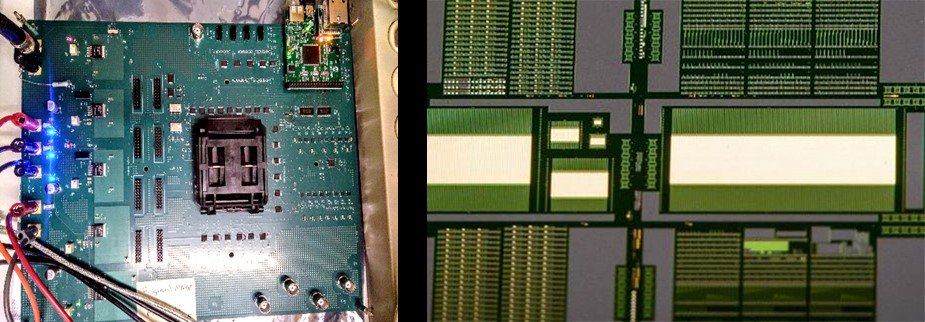
\includegraphics[width=0.65\linewidth]{graphics/Bilder_physische_beschleuniger.jpg}
    \caption{Physical and microscopic view of the mem-HNN}
\end{figure}
\subsection{Hopfield Network}

A Hopfield Network is an \ac{EBM} and belongs to the field of recurrent neural networks.\footcite[cf.][35]{dramschChapterOne702020}
Because the Hopfield Network is the underlying structure of the physical \ac{mem-HNN} accelerator this model is explained first.
The structure of the network consists of only one single layer with binary valued neurons inside.\footcite[cf.][7]{ahadNeuralNetworksWireless2016}
Therefore, the neurons state can either be \{1, 0\} or \{1, -1\}.
The connections between the neurons are symmetrical, which means that the weights of the connections are the same in either direction.\footcite[cf.][7]{ahadNeuralNetworksWireless2016}
Initially, the primary applications of this type of network were to serve as storage for associative patterns and to facilitate pattern retrieval.\footcite[cf.][2]{ramsauerHopfieldNetworksAll2021}
In practive given a query pattern a Hopfield Network can retrive a pattern that is most similar or an is an average of similar patterns.\footcite[cf.][2]{ramsauerHopfieldNetworksAll2021}
In this paper the Hopfield Network's update function interests us because it possibly could be used to sample the intractable training of a \ac{RBM} mentioned earlier.
Surprisingly, since Hopfield networks were introduced by J.J Hopfield in 1982 the storage capacity got increased over time but the fundamentals stayed the same.\footnote{cf.\cite{hopfieldNeuralNetworksPhysical1982}, p. 2554-2558; cf.\cite{ramsauerHopfieldNetworksAll2021}, p. 2}
In following figure 6 an example of a Hopfield Network can be seen.\footcite[cf.][1-2]{yaoMassivelyParallelAssociative2013}

\begin{figure}[H]
    \centering
    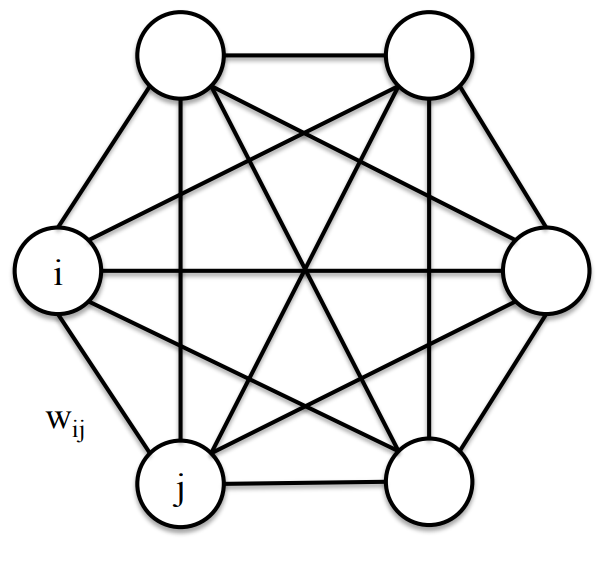
\includegraphics[width=0.3\linewidth]{graphics/Hopfield_Netzwerk.png}
    \caption{Figure of a hopfield network}
\end{figure}
The exemplary network has 6 neurons and bidirectional weigths \( W_{ij} \) between the neurons. 
In addition to that, a Hopfield network has no input or output layer.\footcite[cf.][3]{yaoMassivelyParallelAssociative2013}
The main goal is to find the values for each neuron in the network given a specific input that minimizes the total energy of the system.\footcite[cf.][7]{ahadNeuralNetworksWireless2016}
The minimum energy is then equal to the state where the network is able to perform as a memory item.\footcite[cf.][7]{ahadNeuralNetworksWireless2016}
This energy state can be calculated with the following energy equation\footcite[cf.][2556]{hopfieldNeuralNetworksPhysical1982}: 

\begin{equation}
    E = -\frac{1}{2} \sum_{i \neq j} T_{ij} V_i V_j .
\end{equation}
This energy function invented by Hopfield has big similarities with a \ac{BM} when comparing to the
equation 2.4. This is one of the reasons why the execution on the \ac{mem-HNN} could work out.
When comparing a Hopfield Network, they seek to achieve the effect of changing node activation on the overall energy of the network but \ac{BM}s replace this with the probability of a certain node being activated on the network energy.\footcite[cf.][7]{ahadNeuralNetworksWireless2016}
The second important reason to research the hopfield networks is for their updating process.
Approximately, the activation rule for each neuron is to update its state as if it were a single neuron with the threshold activation function.\footcite[cf.][506]{mackayInformationTheoryInference2003}
\begin{equation}
    s_i \leftarrow 
    \begin{cases} 
    +1 & \text{if } \sum_j w_{ij} s_j + b \geq \theta_i, \\
    -1 & \text{otherwise}.
    \end{cases}
    \label{eq:update_rule}
\end{equation}
    
The state of the neuron will be updated to 1 if the sum over all weights multiplied with the states \{1, -1\} added to a bias \( b \)  is greater than the threshold \( \theta_i \).
In the case of our accelerator the threshold is set to 0 but in theory can be used as an hyperparameter.

Since every neuron's output is an input to all the other neurons the order of the updates need to be specified.\footcite[cf.][506]{mackayInformationTheoryInference2003}
There is the possbility to update all neurons synchronous or asynchronous. 
There is no study that shows what update method leads to better results.
Therefore, this paper follows the asynchronous option first and ensures to do enough sampling steps, so that every neuron has at least updated once before moving on. 

\subsection{Memristor Crossbar Array}

Having set the foundational knowledge about the function of a Hopfield Network the mode of operation can be tackled. 
Since the \ac{mem-HNN} saw the light of day in 2021, a number of improvements have been made to it and at the end of 2023 the individual components can be seen in following figure\footcite[cf.][2]{hizzaniMemristorbasedHardwareAlgorithms2023}:
\begin{figure}[H]
    \centering
    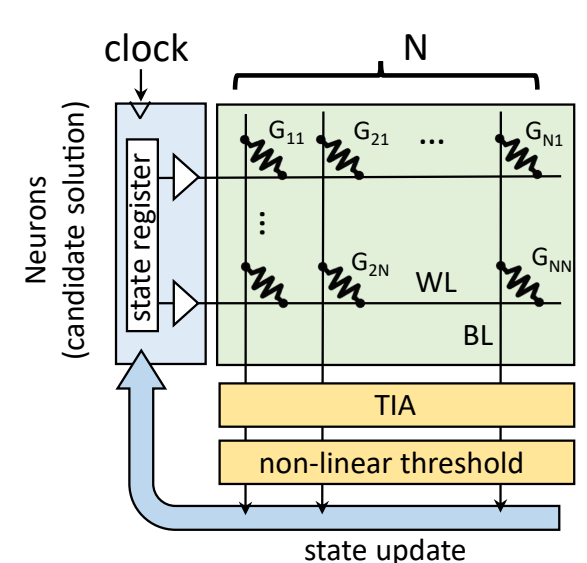
\includegraphics[width=0.3\linewidth]{graphics/Mem_HNN_Modell.png}
    \caption{Modell of the mem-HNN}
    \label{ModellHMM}
\end{figure}
The green square symbolizes the memristor crossbar array, which has the task of performing the in-memory-vector matrix multiplication. 
This is the core part of the architecture that is built around the update formula of the Hopfield Network. 
The memristor crossbar array gets his name because it consists of \textbf{memristors} that connect orthogonal \textbf{electric tracks} with each other.
The \( G_{ij} \) stands for conductance and represents the inverse of the resistance \( R \) of the memristors since \( G = \frac{1}{R}\). On the other hand, \( BL \) (Bitline) and \( WL \) (Wordline) represent the electical tracks.
All the other parts of the model are handled in subchapter 2.4.3, so for now the spotlight belongs to the memristor crossbar array (green square).
A better perspective of the memristor crossbar array gives following 3D model\footcite[cf.][410]{caiPowerefficientCombinatorialOptimization2020}:
\begin{figure}[H]
    \centering
    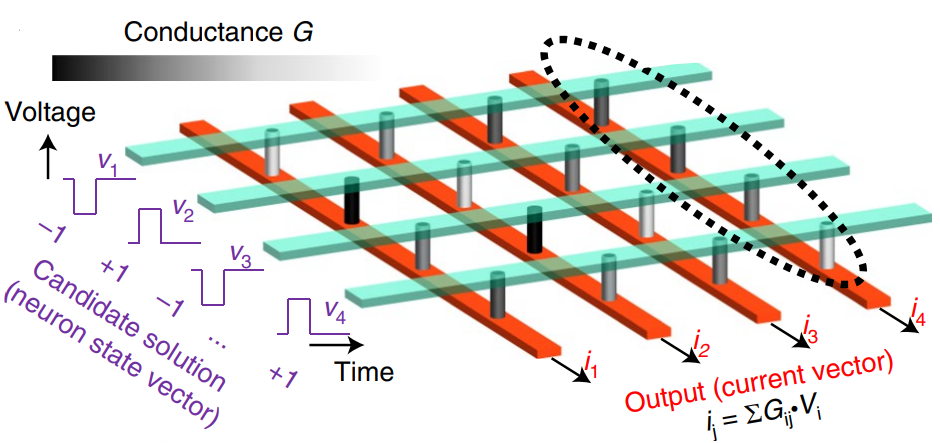
\includegraphics[width=0.65\linewidth]{graphics/memristor_crossbar_array.png}
    \caption{3D modell of the memristor crossbar array}
\end{figure}
To understand how this crossbar array implements the Hopfield network, it helps to have another look at the earlier introduced update formula in equation~\ref{eq:update_rule}.

First of all, on the green Wordline a voltage which either is \( +1 \) or \( -1 \) that represent the state of the neurons in the hopfield network is applied.
Then, the current is flowing towards the memristors, which is an electronic device that functions as a resistor, but with the ability to dynamically change its resistance while the device is being used.\footcite[cf][124]{sungPerspectiveReviewMemristive2018}
In this model the gray cylinders represent the memristors.
The memristors are suitable for matrix vector multiplication because they can use their dynamical resistance to act as weigths.\footcite[cf][124]{sungPerspectiveReviewMemristive2018}
In addition to that, this is the reason why this kind of memory has the potential of high switching speeds, high energy efficiency and high endurance.\footcite[cf.][3]{amirsoleimaniInMemoryVectorMatrixMultiplication2020}

In eletrical terminology, if the resistence of a memristor is higher, the conductance is low since the current can barely flow into the lower Bitlane.
For each of the intersections, when a Wordline meets the crossbar it represents the multiplication of \(w_{ij}\) and \(s_j\) within the update formula.
After the matrix vector multiplication the single currents flow in the same direction on the Bitline and are summed up together with their individual current strength.\footcite[cf.][3]{amirsoleimaniInMemoryVectorMatrixMultiplication2020}
The reason for this phenomenon is the 1. Kirchhoff'sche rule, which is not further explained here since it would be out of scope.
To make an example for each output current \(i_{1}\) has for intput voltages \(V_{1}, V_{2}, V_{3}, V_{4}\).
The current flowing into the lower Bitlane is now according to Ohm's rule \( i_{out} = \frac{1}{R_{memristor}} * V_{in}\).
Since \( G = \frac{1}{R}\) and Kirchhoff'sche rule sums up each current \(i\) is \( i_{1} = G_{11}*V_1 + G_{12}*V_2 + \cdots + G_{14}*V_4\)
As a result the first first part \(\sum_j w_{ij} s_j\) of the updating formula of the Hopfield Network is established.
Last but not least, adding the bias \(b\) to the sum is achieved by simply adding an intial current, which is worth the amount of the bias, to the the total Bitline current.
Each i is the output of the current vector and equal to a neuron within the Hopfield Network with all the memristors on this lane symbolizing the weights that all the other neurons connect to it.

The way the memristors work is to imagine them as plate capacitors. 
The following figure shows how memristors function achieve the dynamically changing resistance.\footnote{\cite{changDirectObservationDualFilament2017}, p. 6; \cite{sungPerspectiveReviewMemristive2018}, p. 2}
\begin{figure}[H]
    \centering
    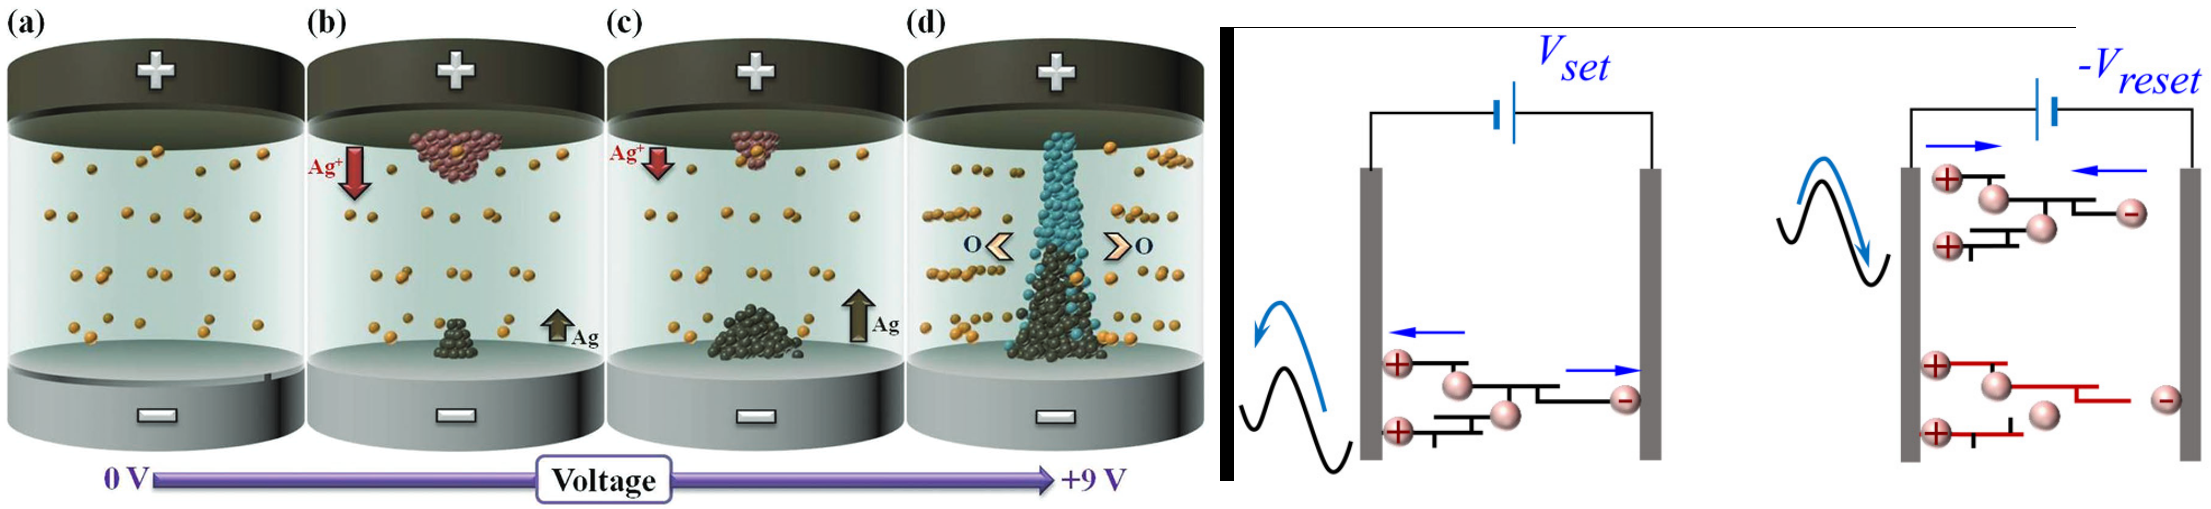
\includegraphics[width=0.9\linewidth]{graphics/Memristor_filoments.png}
    \caption{Memristor-based learning}
    \label{platecondensator}
\end{figure}

Essentially, the memristor consists out of two metal electrodes and a dielectric layer that is sandwiched between them.\footcite[cf.][1]{changDirectObservationDualFilament2017}
In case of the \ac{mem-HNN} it is an oxide memristors that uses tantalum oxide (TaOx) and oxygen atoms as dielectric layer.\footcite[cf.][412]{caiPowerefficientCombinatorialOptimization2020}
Initially the metal-ions are freely moving within the dielectric layer. 
A visual representation can be observed in section \(a)\) on the left side of \ref{platecondensator}.
In \textbf{phase 1}, the programming phase, an electrical field is applied to the plate capacitors which leads to the formation of a conductive filament within the dielectrive layer.\footcite[cf.][3]{changDirectObservationDualFilament2017}
The conductive filament can be imagined as a string, which is formed out of the metal-ions.
Therefore, they are able to conduct electricity once they built.\footcite[cf.][5]{changDirectObservationDualFilament2017}
This process, visualized from \(a)-d)\), can be controlled due to the voltage that is aplied to the memristor.
Wigh a high enough voltage a filament can be established and increasing the voltage from there on ensures that even stronger and thicker filaments are created.
This in fact is the explanation on how the resistance of the memristor can change dynamically and is able to store the information
about the preferred conductance. A schematic view of the filament and phase 1 is also shown in the right part of \ref{platecondensator}, where the label is \(V_{set}\) 
An everyday example would be a water pupe with a valve that can be adjusted to control the water flow. 
The vavle symbolizes the memristor and the water flow the current in the electrical tracks.
On the actual \ac{mem-HNN} there is a controller, which is not shown in the model, that talks to a digital external computer that gives the inforation on hot to chose \(V_{set}\) for each memristor.

In \textbf{phase 2}, the performing phase, the electrical field is removed.
Now, the filament has reached its final form and is not able to grow anymore but most importantly it stays the same.\footcite[cf.][1-2]{sungPerspectiveReviewMemristive2018}
The filament connects the top and bottom metal electrodes of the memristor with each other.
The enduring presence of a filament in the memristor, even without an applied voltage, embodies its namesake combination of memory and resistor.
As a result in this phase the workload can be executed and the memristor has the desired conductance.

The final \textbf{phase 3} is the dissolution of the filament to readjust the resistance for the next iteration.
This process is called bipolar switching and a schematic view of it is shown in the right part of \ref{platecondensator}, where the label is \(-V_{reset}\).
Filament disonnection is performed through ionic switching, which works by swapping the plus and minus poles around.
Next up, the filament wants to rearrange and disconnects from top and bottom of the metal electrodes. 
Since this process of establishing the filaments (setting the desired resistance) and disconnecting them (preparing for new desired resistanc) this process is called bipolar switching.\footcite[cf.][7]{sungPerspectiveReviewMemristive2018}

Presently, the research on the application of memristor crossbar arrays in supervised learning is sparse, indicating a clear necessity for further investigative studies to understand their potential and usability.\footnote{cf.\cite{amirsoleimaniInMemoryVectorMatrixMultiplication2020}, p. 8; cf.\cite{sungPerspectiveReviewMemristive2018}, p. 124}
In the practical part exactly this is put to the test and training data of the \ac{RBM} should be generated to give clearance about the feasibility of this idea.
A possbility is to use the memristor to set the resistance \(V_{set}\) for one training iteration with the needed weigths, reset them \(-V_{reset}\) and 
initiate the following training with the new weights that are digitally updated. 

\subsection{Output Hopfield Network}

In this subchapter the left over components of the \ac{mem-HNN} shown in \ref{ModellHMM} are adressed.
To remain in the correct sequence, after the memristor crossbar array the \ac{TIA} is addressed next.
The \ac{TIA} is the component that converts the current \(i_j\), which is the output of the memristor crossbar array, into a voltage. \footcite[cf.][3]{hizzaniMemristorbasedHardwareAlgorithms2023}
Since each output current symbolizes one neuron, there are also that many \ac{TIA}s required.

Subsequently, to fulfill the update formula of the Hopfield Network, that the \ac{mem-HNN} impersonates, is the non-linear threshold.
The non-linear threshold is used to compare the \(\sum_j w_{ij} s_j + b\) against the threshold \(\theta_i\) to determine whether it is \(\geq\) or \(<\).\footcite[cf.][18]{caiHarnessingIntrinsicNoise2019}
In terms of electrical components the non-linear threshold is a comparator. 
A voltage comparator is an analog electronical device.
Comparators are able to compare a input signal, which is the converted voltage of the \ac{TIA}, with a reference voltage, which is the threshold \(\theta_i\).\footcite[cf.][28]{chenApplicationVoltageComparator2021}
In addition to that, the comparator is the component that transforms the analog voltage into a binary digital signal.
The digital signal is a binary voltage and either is \(0V\) or if the sum was greater than the threshold it is a specific voltage \(V_{out}\).
The output represents the new state of a neuron in terms of the Hopfield Network and is now trasmitted to the state register.

The state register is a digital memory that is designed to store the current neuron configuarion (input vector).\footcite[cf.][18]{caiHarnessingIntrinsicNoise2019}
The binary states of the neurons, which represent the voltage output of the comparator, are sent to the state register and update the old configuration.\footcite[cf.][3]{caiHarnessingIntrinsicNoise2019}
For each neuron there is one \ac{TIA} and an according comparator required. 
This not only allows for fast parallel computation but also it allows to exactly map the digital output of the comparator to the correct position within the state register.
Now, a new sampling step can begin and neurons states can be updated. 

A missing component part in figure\ref{ModellHMM} is a selector that is connected to the state register. 
Its task is to allow updating through unlockickt the correct positions inside the state registor.  
For example the mode of updating can be selected with either one neuron updated at a time asynchronously or multiple neurons synchronous. 
A promissing and interesting sampling strategy could be to update \(N/2\) of all neurons.\footcite[cf.][3]{hizzaniMemristorbasedHardwareAlgorithms2023}
So when there are 100 neurons in the neural network with each sampling step 50 neurons are updated.

The white arrows next to the state register in figure\ref{ModellHMM} represent a Wordline driver. 
Wordline Drivers are a voltage source that determines the voltage by the state of the state register.
They are required to enable a parallel activation of Wordlines and to start the new sampling step.\footcite[cf.][18]{caiHarnessingIntrinsicNoise2019}

Finally, it is worth to mention one sampling step can happen within one clock cycle of the. 
There are thousands of sampling iterations that are performed within one training iteration of a neural network.
After each sampling iteration the neuron configuration in the state register is saved either in a cache directly on the \ac{ASIC} hardware or
sent to a digital external computer. 
For example after 10000 sampling iterations the arrays of the hidden- and visible neurons are sent to the computer to perform a prediction after the iteration.
This completes the explanation of how the \ac{mem-HNN} implements the concept of a Hopfield Network. 


\subsection{Noisy Hopfield Network}

Currently, the \ac{mem-HNN} is also able to use noise injection to ensure the chance of finding a low energy minima of the Ising problem.
This noise injection happens between the output of the Bitline and the \ac{TIA}. 
The noise enables to escape local minmina of the energy landscape and to find lower energy minimas or even the global minima, which is equal to the solution of the optimization problem and therefore improves solution quality anf effciency.\footcite[cf.][410]{caiPowerefficientCombinatorialOptimization2020} 
This is achieved by a random number generator in the hardware that creates a random array filled with digital signals.\footcite[cf.][22]{caiHarnessingIntrinsicNoise2019}
Out of this array a \ac{DAC} takes a subset of this array and converts them into a floating point noise signal for each neuron.\footcite[cf.][3]{hizzaniMemristorbasedHardwareAlgorithms2023}
This noise injection uses the created floating point noise signal and adds it to the update formula.
Effectively the new noisy hopfield network updating function now looks like the following: 
\begin{equation}
    s_i \leftarrow 
    \begin{cases} 
    +1 & \text{if } \sum_j w_{ij}  + b + \mathbf{n} \geq \theta_i, \\
    -1 & \text{otherwise}.
    \end{cases}
\end{equation}
with \(n\) representing the noise.\footcite[cf.][410]{caiPowerefficientCombinatorialOptimization2020} 
Besides aiding optimization tasks, noise also creates an interesting link to \c{BM}s.
Without noise the Hopfield Network is only able to do perform optimization tasks and no sampling, which is needed to train a \ac{RBM}.
The difference between the \ac{RBM} and the Hopfield Network without noise is the activation function.
As shown in equation \ref{eq:update_rule}, a simple Hopfield Network has no temperature and has a binary step function as activation function which is completely deterministic.
In contrast, a \ac{RBM} has a statistical logistic sigmoid function as activation function shown in figure \ref{logistic_sigmoid}, which uses a temperature of \(1\) mentioned in 2.2.4.
Therefore, to successfully implement a \ac{RBM} on the \ac{mem-HNN} the activation behavior of the neurons need to be compatible with the activation function of the \ac{mem-HNN}.

A potential solution to address the issue of activation behavior and enhance compatibility involves utilizing noise from an analog noise source.\footnote{cf.\cite{bohmNoiseinjectedAnalogIsing2022}, p. 1-2; cf.\cite{mahmoodiVersatileStochasticDot2019}, p. 2}
One relatively straightforward way to inject noise into the activation function is by adding a normal gaussian distribution \(g(x)\) on top of it\footcite[cf.][3]{bohmNoiseinjectedAnalogIsing2022}:
\begin{equation}
    f_g(x) = \frac{1}{\sqrt{2\pi\rho^2}} e^{-\frac{(x-\mu)^2}{2\rho^2}},
\end{equation}
with \(\rho\) representing the standard deviation and \(\mu\) represents the mean of the distribuion.
The visual representation of a gaussian distribution is shown in following figure. 
It illustrates distributions with different parameters of the standard deviation and the mean of the distribution allowing for a better understanding of the flexibility and possbilities of noise injection. 
\begin{figure}[H]
    \centering
    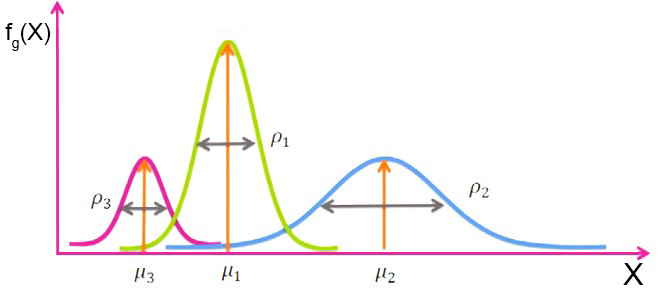
\includegraphics[width=0.65\linewidth]{graphics/Gaussian_Normal_Distribution_edited.jpg}
    \caption{Gaussian normal distribution\protect\footnotemark}
    \label{normalGaussianDistribution}
\end{figure}
\footnotetext{modified from \cite[cf.][3]{gmComprehensiveSurveyAnalysis2020}}
There have been recent proposals that show a proof of concept on how to inject the noise with a gaussian distribution and make a \ac{RBM} realizable.\footnote{cf.\cite{bohmNoiseinjectedAnalogIsing2022}, p. 1-2; cf.\cite{mahmoodiVersatileStochasticDot2019}, p. 2}
In the paper by Böhm et al., they used analog singals for the neurons instead of digital signals like the \ac{mem-HNN} uses. 
Furthermore, they used an opto-electrical Ising machine in combination with an \ac{FPGA} as accelerator which works in a similar fashion to the \ac{mem-HNN}.\footcite[cf.][1-11]{bohmNoiseinjectedAnalogIsing2022}

The second paper by Mahmoodi/Preziosi and Strukov, also created a proof of concept in which they showed an implementation of a \ac{RBM} on a memristor crosbar array.
Crucially, there is no state registor or comparator involved, so all the calculations of comparing against a threshold, adding a bias and adding the noise were made by an external digital computer. 
The hardware computes solely the matrix vector multiplication.
Hence, the additional required interfaces make the system slow and inefficient.\footcite[cf.][1-8]{mahmoodiVersatileStochasticDot2019}

However, beyond these initial proof of concepts, it is still an open question if the concept
is feasible on the complete \ac{ASIC} hardware accelerator like the \ac{mem-HNN} and if it does bring an actual acceleration of the training and interference of a \ac{RBM}.
